\documentclass[11pt]{article}

% --------------------
% Template settings (do not change: 11pt, 1in margins, 1.10 stretch)
% --------------------
\usepackage[margin=1in]{geometry}
\usepackage{amsmath,amssymb}
\usepackage{array}
\usepackage{booktabs}
\usepackage{enumitem}
\usepackage{xcolor}
\usepackage{setspace}

% --------------------
% Extra packages used by our report
% --------------------
\usepackage{graphicx}
\usepackage{float}
\usepackage{caption}    % \captionof for the side-by-side figure + table
\usepackage{tabularx}
\usepackage{tikz}
\usepackage{listings}
\usepackage[numbers]{natbib}
\usepackage{hyperref}   % keep last

\setstretch{1.10}
\setlength{\emergencystretch}{2em}

\hypersetup{
    colorlinks=true,
    linkcolor=blue!50!black,
    urlcolor=blue!50!black,
    citecolor=black
}

% Float placement: let figures share pages with text instead of
% leaving half-empty float pages (does not touch font, margins or spacing)
\renewcommand{\topfraction}{0.9}
\renewcommand{\bottomfraction}{0.8}
\renewcommand{\textfraction}{0.1}
\renewcommand{\floatpagefraction}{0.8}
\setcounter{topnumber}{3}
\setcounter{totalnumber}{5}

\usetikzlibrary{positioning,arrows.meta}
\graphicspath{{figures/}}

% JSON listing style (appendix)
\lstdefinelanguage{json}{
    morestring=[b]",
    stringstyle=\color{blue!55!black},
    morekeywords={true,false,null},
    keywordstyle=\color{purple!65!black},
    sensitive=false,
    showstringspaces=false
}
\lstdefinestyle{jsonstyle}{
    language=json,
    basicstyle=\ttfamily\scriptsize,
    breaklines=true,
    breakatwhitespace=false,
    columns=fullflexible,
    keepspaces=true,
    frame=single,
    rulecolor=\color{black!20},
    backgroundcolor=\color{gray!3},
    numbers=left,
    numberstyle=\tiny\color{gray},
    numbersep=7pt,
    xleftmargin=12pt,
    framexleftmargin=8pt,
    tabsize=2,
    showstringspaces=false,
    captionpos=b
}

% --------------------
% Course information
% --------------------
\newcommand{\course}{DSA4213: Natural Language Processing for Data Science}
\newcommand{\semester}{Semester 1, AY2026/2027}

\begin{document}

\begin{center}
{\LARGE\bfseries Group Project Final Report}\\[0.4em]
{\large Beyond Retrieval: Scope-Aware Memory Application in AI Agents}\\[0.9em]
Group ID: 3\\[0.9em]
\course\\
\semester
\end{center}

% ====================
% Administrative information
% ====================
\section*{Administrative Information}

\begin{tabular}{@{}>{\bfseries\raggedright\arraybackslash}p{0.25\linewidth}
                    >{\raggedright\arraybackslash}p{0.70\linewidth}@{}}
Group members & Isaac Chin Wei En (A0248885H),
Edward Chew Kian Boon (A0271710N),
Ng Cheng Kiat Nicholas (A0271938R),
Jagan Mohan Shailesh (A0272542H) \\[0.7em]
Project direction & Do agents with memory act on the right memory when a
project-specific instruction conflicts with a general preference,
and whether labelling memories by scope helps. \\[0.7em]
Repository & Link to the code and project materials: \url{https://www.github.com/jmshai/dsa4213-project-code} \\
\end{tabular}

% ====================
% Project summary (original abstract)
% ====================
\section*{Project Summary}

Long-term memory enables language-model agents to retain user
preferences across interactions, but retrieving a relevant memory
does not guarantee that the agent applies it in the correct context.
We investigate scope-aware memory application by augmenting Mem0
and Supermemory with write-time and read-time scope tagging.
We construct a benchmark of 40 episodes in 20 paired scenarios,
covering five types of conflicting instructions, and evaluate eight
conditions across 320 runs. The expected memory was retrieved in
43 of 51 incorrect responses across the six memory-system conditions,
demonstrating a substantial retrieval--application gap. Read-time
tagging with Supermemory achieves the highest observed adherence
(92.5\%), compared with 85\% for its baseline (not statistically
significant, $p=0.25$), while write-time tagging reduces adherence
for both systems. These findings suggest
that explicit scope information can support memory application,
but its effectiveness depends on how it is integrated and used.

% ====================
% 1. Problem, research question, and motivation
% ====================
\section{Problem, Research Question, and Motivation}
\label{sec:introduction}

\subsection{Motivation and Research Problem}

Memory-augmented language-model agents retain user instructions
across conversations, allowing responses to reflect previously
expressed preferences. However, preferences are not always
universally applicable: a user may generally prefer Polars for
large datasets while requiring pandas for a particular group
project. Both memories remain valid, but the appropriate action
depends on the current context.

Existing memory systems primarily address the storage and
retrieval of relevant information. Yet even when conflicting
instructions are successfully retrieved, an agent must determine
which instruction applies, whether an exception overrides a
standing preference, and whether a temporary instruction should
continue to influence subsequent tasks.

We investigate this distinction between \emph{memory retrieval}
and \emph{memory application}: does an agent correctly use a
retrieved instruction within its intended scope, and can providing
explicit information on the memories' scopes improve its decisions?

\subsection{Research Objectives and Contributions}

We investigate two questions: (1) whether agents make incorrect
decisions despite retrieving the expected memory, and (2) whether
scope-aware interventions improve contextual adherence while
preserving unrelated preferences.

Our contributions are:
\begin{enumerate}
    \item A lightweight scope-tagging layer supporting standing,
    project-specific, and single-task instructions, integrated
    with Mem0 and Supermemory at write time or read time.
    \item A synthetic benchmark of 20 paired scenarios (40
    episodes) covering five memory-conflict categories.
    \item An evaluation of eight conditions across 320 runs,
    separating retrieval success, memory application, scope
    errors, tagging accuracy, and unrelated-memory retention.
\end{enumerate}

% ====================
% 2. Related work and contribution
% ====================
\section{Related Work and Contribution}
\label{sec:related}

\subsection{Long-Term Memory in LLM Agents}

Mem0~\cite{chhikara2025mem0} provides persistent agent memory
through extraction, storage, updating, and retrieval of
information from interactions. Supermemory
\cite{supermemoryresearch} offers a hosted memory service with
ingestion and semantic search. Both make prior information available to agents without
resupplying full conversation histories.

We use these systems as memory backends rather than proposing
another storage or retrieval mechanism, and evaluate whether
their retrieved information supports contextually appropriate
decisions.

\subsection{Memory Retrieval and Contextual Applicability}

Retrieval relevance and contextual applicability are distinct.
A memory may be relevant to the current topic but inapplicable
to the current project, task, or condition. Conversely, a
retrieved exception may need to override a broader preference
without permanently replacing it.

We focus on this downstream decision problem, representing
scope explicitly and evaluating both correct application and
application beyond a memory's intended context.

% ====================
% 3. Agent and task setup
% ====================
\section{Agent and Task Setup}
\label{sec:experimental-setup}

\subsection{Implementation and Model Configuration}

The agent is
\texttt{qwen/qwen3.8-flash} through OpenRouter, with
temperature 0, seed 4213, a 1,024-token output limit,
and reasoning disabled. The agent prompt template and
sampling settings are fixed across conditions, with
retrieval limited to ten results.

Qwen was selected after an operational pilot: it
reported zero reasoning usage on 40 pilot calls,
whereas DeepSeek returned empty text on three of
eight calls when reasoning was disabled.

Both memory systems use a common interface and fresh
namespaces for each episode and condition. Mem0 uses
its default extraction and search with a local embedder
and vector retrieval without BM25; Supermemory uses its
hosted API and waits for ingestion before retrieval
(details in Appendix~\ref{app:reproducibility}).


\subsection{Experimental Conditions and Baselines}
\label{sec:conditions}

We evaluate eight conditions: no memory (current probe only),
full transcript (all earlier sessions), Mem0 and Supermemory
with native retrieval, and write-time (pre-extracted, tagged
memories) and read-time (retrieved memories tagged afterward)
scope-tagged variants of each memory system.

Each condition runs all 40 episodes (320 runs). The scope-layer
conditions change tags, resolution rules, and memory ordering
together, so their effects cannot be isolated.


% ====================
% 4. System or study design
% ====================
\section{System or Study Design}
\label{sec:methodology}

\subsection{Scope Representation and Conflict Resolution}
\label{sec:scope-representation}

Each instruction is represented by three fields:
\emph{scope}, \emph{key}, and \emph{condition}.
The scope determines applicability, the optional key identifies
a project or task, and the optional condition specifies an
additional constraint.

\begin{table}[t]
\centering
\small
\caption{Scope representation.}
\label{tab:scopes}
\begin{tabularx}{\linewidth}{lXl}
\toprule
Scope & Applicability & Example \\
\midrule
Standing & General preference across tasks &
Use Polars \\
Project & Restricted to a named project &
Marlin: pandas \\
Single-task & Restricted to one task &
This export: CSV \\
\bottomrule
\end{tabularx}
\end{table}

The reference decision policy first excludes memories whose
project, task, or condition does not match the current request.
Among applicable memories concerning the same decision, scope
precedence is
\[
\text{single-task} \succ \text{project}
\succ \text{standing}.
\]
Within one scope, an applicable conditional instruction takes
precedence over an unconditional instruction; recency resolves
remaining conflicts at equal specificity. Unrelated instructions
do not compete, and the benchmark excludes unresolved ties.

These rules define the reference actions and are communicated
to the agent. The scope layer does not deterministically
select the winning memory.

\subsection{Scope-Tagging Architecture}
\label{sec:architecture}

We augment Mem0~\cite{chhikara2025mem0} and
Supermemory~\cite{supermemoryresearch} with an LLM-based
scope tagger. Figure~\ref{fig:architecture} compares the
two integration strategies.


\begin{figure}[t]
\centering
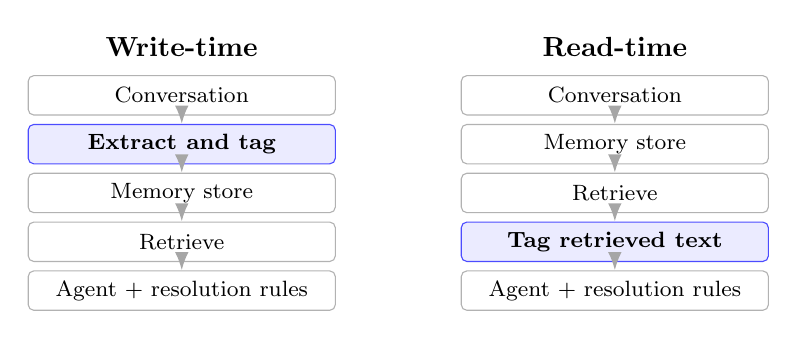
\begin{tikzpicture}[yscale=0.62,
    >=Latex,
    node distance=0.55cm,
    box/.style={
        draw=gray!60,
        rounded corners=2pt,
        minimum width=3.9cm,
        minimum height=0.5cm,
        align=center,
        font=\footnotesize
    },
    tag/.style={
        box,
        draw=blue!70,
        fill=blue!8,
        font=\footnotesize\bfseries
    },
    arrow/.style={->,thick,gray!70}
]

% Column headings
\node[font=\bfseries] at (0,0) {Write-time};
\node[font=\bfseries] at (5.5,0) {Read-time};

% Write-time pipeline
\node[box] (w1) at (0,-1) {Conversation};
\node[tag] (w2) at (0,-2) {Extract and tag};
\node[box] (w3) at (0,-3) {Memory store};
\node[box] (w4) at (0,-4) {Retrieve};
\node[box] (w5) at (0,-5) {Agent + resolution rules};

% Read-time pipeline
\node[box] (r1) at (5.5,-1) {Conversation};
\node[box] (r2) at (5.5,-2) {Memory store};
\node[box] (r3) at (5.5,-3) {Retrieve};
\node[tag] (r4) at (5.5,-4) {Tag retrieved text};
\node[box] (r5) at (5.5,-5) {Agent + resolution rules};


% Write-time arrows
\draw[arrow] (w1.south) -- (w2.north);
\draw[arrow] (w2.south) -- (w3.north);
\draw[arrow] (w3.south) -- (w4.north);
\draw[arrow] (w4.south) -- (w5.north);

% Read-time arrows
\draw[arrow] (r1.south) -- (r2.north);
\draw[arrow] (r2.south) -- (r3.north);
\draw[arrow] (r3.south) -- (r4.north);
\draw[arrow] (r4.south) -- (r5.north);


\end{tikzpicture}
\caption{Scope-tagging integration strategies.
Write-time tagging occurs before storage, whereas
read-time tagging occurs after retrieval.}
\label{fig:architecture}
\end{figure}


Write-time tagging extracts individual instructions from the
full conversation and stores them with scope metadata. It
can preserve scope cues early but may discard surrounding
conversational context. Read-time tagging operates on the
memory system's retrieved text, preserving native storage
behaviour but relying on that text to retain sufficient
contextual information.

Both strategies supply tagged memories and conflict-resolution
rules to the agent. Structured task identifiers are withheld
from the taggers, so task continuity must be inferred from
natural-language context.

\subsection{Benchmark Construction}
\label{sec:benchmark}

\subsubsection{Episode Structure and Mirrored-Pair Design}

We construct 20 paired scenarios containing 40 episodes.
Each pair includes two or three earlier conversation sessions,
reference memories, and two probes sharing the same history.
Probe A tests an applicable scoped instruction; Probe B
changes the project, task, or condition so that the instruction
no longer applies. Each episode consists of one probe and
its shared history, with an expected action for evaluation.

Each pair also includes an unrelated standing preference and
a retention check. Pair accuracy requires both probes to be
correct, discouraging fixed choices that ignore context.

Appendix~\ref{app:po01-example} (Figure~\ref{fig:mirrored-pair}) walks through pair \texttt{po-01}.

\subsubsection{Conflict Categories and Dataset Generation}

The benchmark covers five conflict categories with four
pairs each, testing project exceptions, temporary task
exceptions, conditional applicability, replacement of older
instructions within one scope, and precedence of more
specific instructions within one scope.

The 20 pairs contain 66 distinct reference memories,
including competing and unrelated instructions.
Nineteen pairs were initially drafted with AI assistance
and subsequently reviewed and revised. The suite varies
domains, wording, chronology, and instruction positions;
some standing preferences deliberately appear after
narrower instructions.

\subsubsection{Dataset Validation and Gold Labels}

Automated checks validate the JSON schema, verbatim
memory quotations, paired-probe similarity, expected
decisions, and diversity. Only session and probe text
reach the systems; structured gold labels and expected
actions are withheld. A leakage test checks this
separation.

The 66 reference memories were independently annotated
by two human annotators for scope, key, and condition.
The annotations were reviewed and reconciled to establish
the final gold labels. After reconciliation, scope and key
labels matched the original drafts, while four
condition-expression differences were reviewed and resolved. 


% ====================
% 5. Evaluation and results
% ====================
\section{Evaluation and Results}
\label{sec:results}

\subsection{Evaluation Metrics}
\label{sec:metrics}

An LLM judge identifies the action taken in each
free-text answer. We report adherence (expected action selected),
pair accuracy (both A and B probes correct), the
retrieval--application gap (expected memory retrieved but wrong
action selected), retention (unrelated standing preference
followed), tag accuracy, and failure stage; Appendix~\ref{app:metrics}
gives the definitions.

Adherence is also separated into in-scope (A) and
out-of-scope (B) probes. Incorrect decisions are
classified as over-application, under-application,
supersession, or other actions.

Retrieval is checked by verbatim or judge-assisted
matching of rewritten notes; the full-transcript control
counts as retrieved by construction, and no memory as not
retrieved. Retention excludes unassessable answers.

Tagging accuracy is measured per field against the gold
labels on notes tied to one reference memory
(Appendix~\ref{app:metrics}).

Each incorrect answer is assigned to its earliest detected
failure stage (extraction, retrieval, scope loss, tagging, or
reasoning). These are diagnostic classifications, not
established causal mechanisms, and Supermemory's internal
extraction cannot be inspected separately from retrieval.

\subsection{LLM-as-a-Judge and Statistical Analysis}
\label{sec:judge}

The judge is the same Qwen model at temperature 0. It sees the
probe, response, and alphabetically ordered candidate actions
(not the expected action) and returns an action,
\texttt{none}, or \texttt{mixed}, with evidence; it also
evaluates the retention check.

The recorded human review covers 40 action labels
and 38 assessable retention labels, with complete
agreement against the judge (Cohen's
$\kappa=1.00$)~\cite{cohen1960coefficient}.
The judge and agent share a model, so correlated
errors remain possible; LLM-judge biases are
discussed by Zheng et al.~\cite{zheng2023judging}.

We report 95\% Wilson confidence intervals
\cite{wilson1927probable} and exploratory exact
McNemar tests~\cite{mcnemar1947sampling} on the
same episodes. Because the A/B probes within a
pair share history, episode-level tests do not
fully account for dependence; p-values are
interpreted cautiously. All 320 runs completed without
execution errors.

\subsection{Overall Correction Adherence}

Figure~\ref{fig:overall-adherence} shows adherence
across the eight conditions. No memory achieves
20\% (8/40), versus 80\% (32/40) with the full
transcript. Mem0 and Supermemory achieve 77.5\%
(31/40) and 85\% (34/40).

Read-time tagging achieves 80\% with Mem0 and
92.5\% (37/40) with Supermemory, the highest
observed score. Write-time tagging reduces
adherence to 60\% and 77.5\%, respectively.
Supermemory + read-time resolves 17/20 complete
pairs, compared with 15/20 for its baseline.
Its improvement is not statistically significant
under the reported McNemar test ($p=0.25$).

\begin{figure}[t]
\centering
\begin{minipage}[t]{0.45\linewidth}
\centering
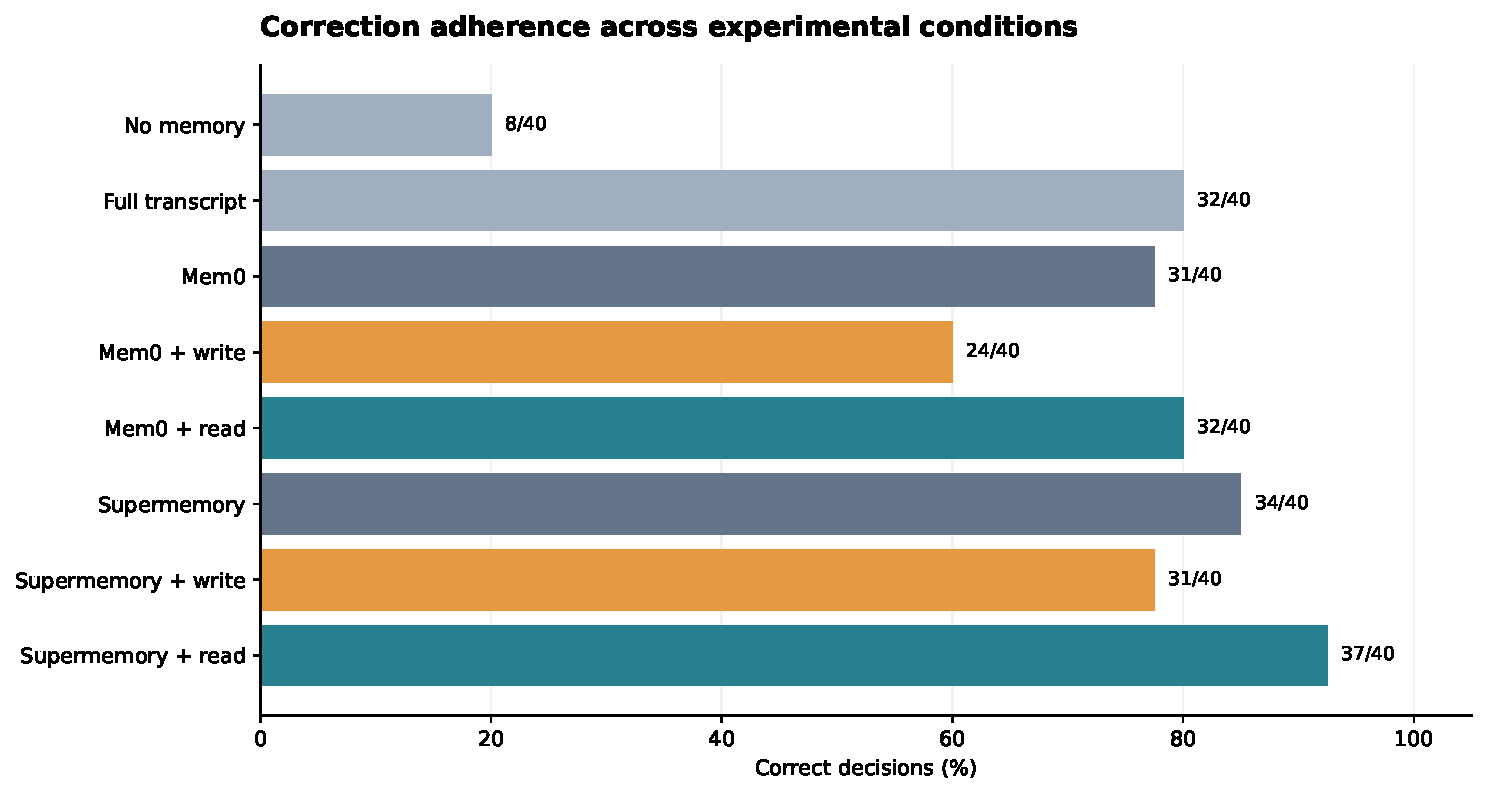
\includegraphics[width=\linewidth]{01_overall_adherence.pdf}
\caption{Correction adherence across eight conditions
(40 episodes per condition); error bars are 95\% Wilson
intervals.}
\label{fig:overall-adherence}
\end{minipage}\hfill
\begin{minipage}[t]{0.45\linewidth}
\centering
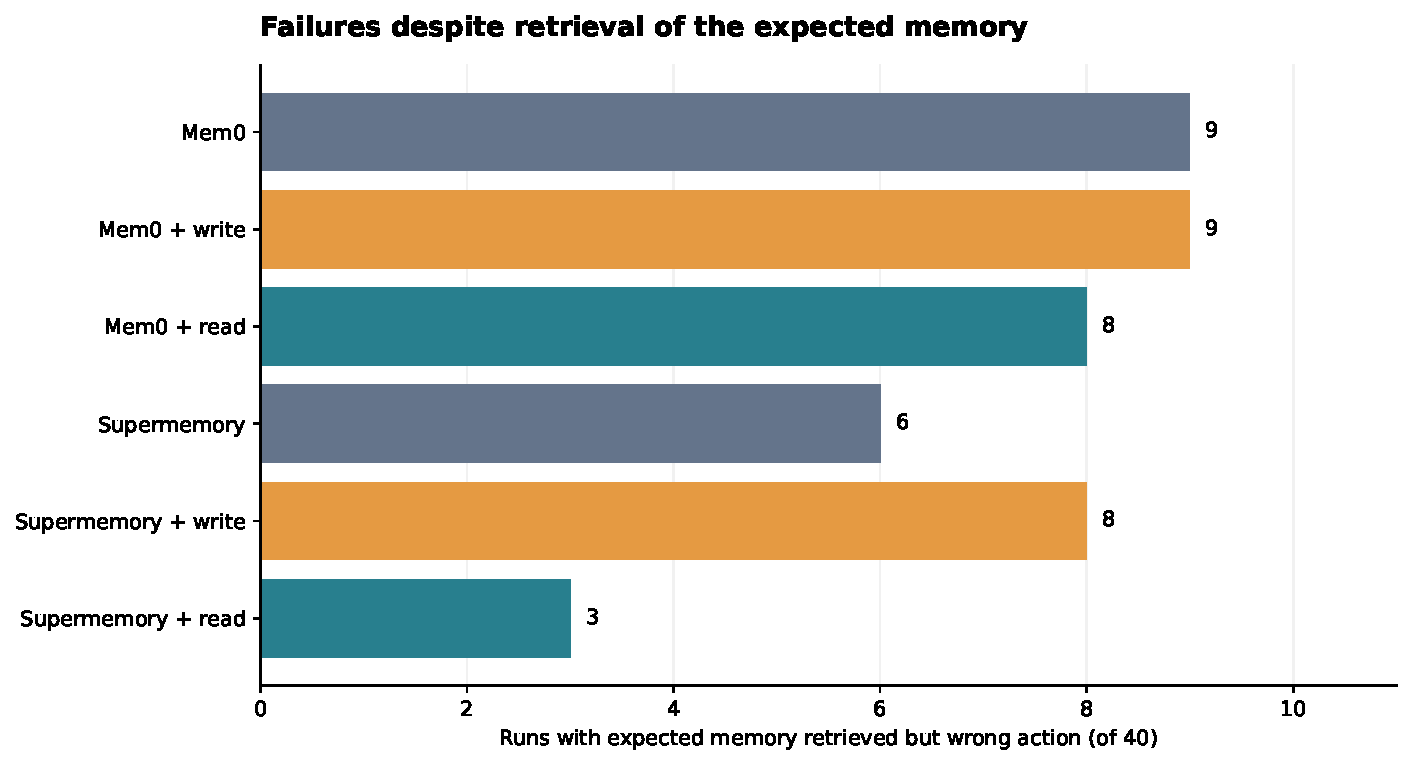
\includegraphics[width=\linewidth]{02_retrieved_but_wrong.pdf}
\caption{Incorrect actions despite retrieval
of the expected memory.}
\label{fig:retrieval-gap}
\end{minipage}
\end{figure}

\subsection{Retrieval Versus Application}

Across the six memory-system conditions, 43 of 51
incorrect responses occurred despite retrieval of
the expected memory (Figure~\ref{fig:retrieval-gap}).
Unmodified Mem0 and Supermemory retrieved the
expected memory in all 40 episodes but made nine
and six incorrect decisions, respectively.
Read-time tagging reduced these counts to eight
and three.

Successful retrieval is thus insufficient for correct
application, although a retrieved note may have lost scope
information.


\subsection{Scope-Boundary and Conflict-Type Performance}

Figure~\ref{fig:scope-boundaries} reveals asymmetric
write-time errors. Mem0 + write correctly handles
10/20 in-scope probes, versus 17/20 for Mem0.
Supermemory + write handles 11/20, versus 18/20
for its baseline, but correctly handles all 20
out-of-scope probes. This indicates substantial
under-application of scoped instructions.

Supermemory + read-time handles 20/20 in-scope
and 17/20 out-of-scope probes.

\begin{figure}[t]
\centering
\begin{minipage}[t]{0.45\linewidth}
\centering
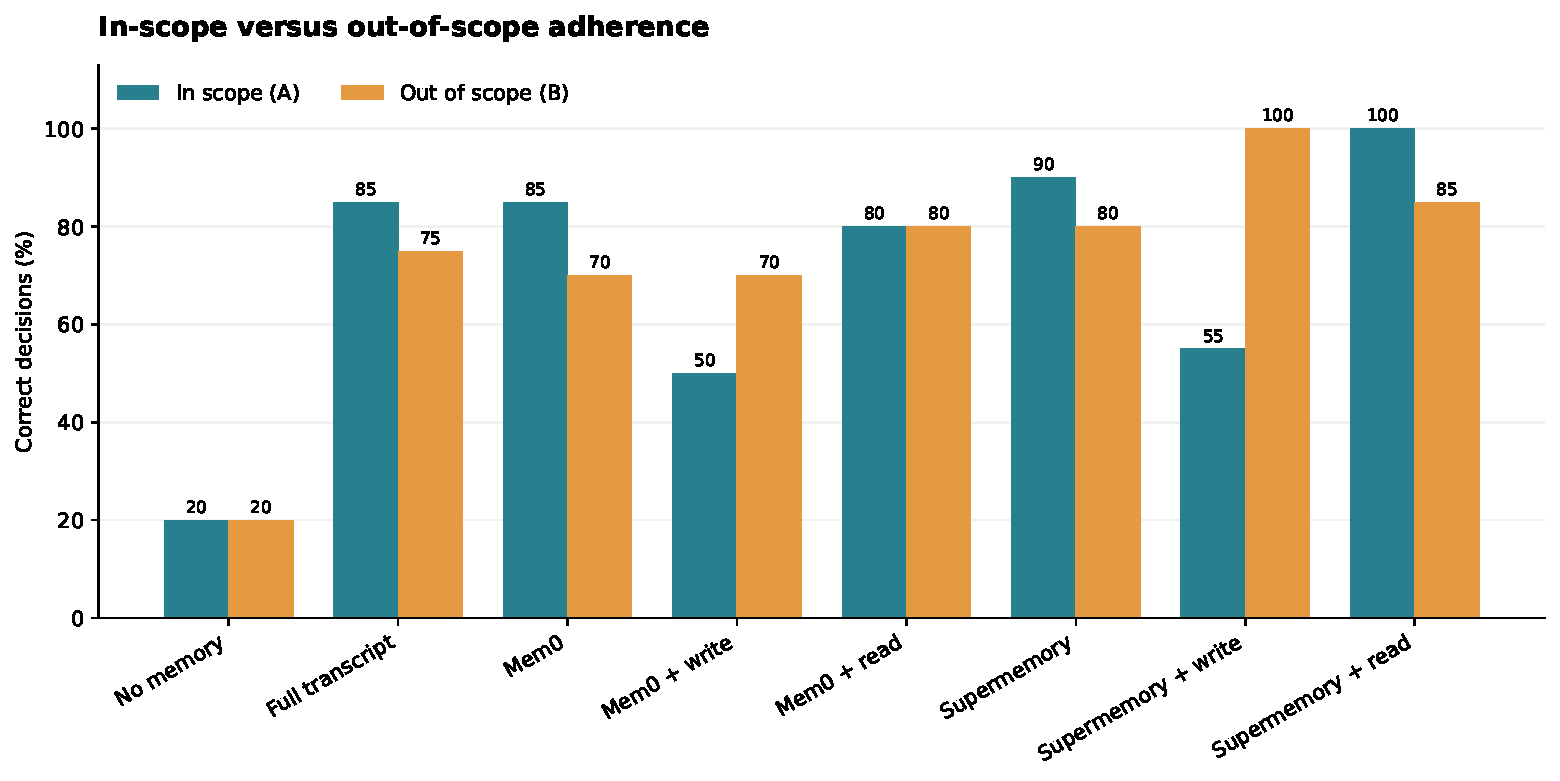
\includegraphics[width=\linewidth]{03_in_scope_vs_out_scope.pdf}
\caption{Adherence on in-scope (A) and out-of-scope
(B) probes, 20 of each per condition.}
\label{fig:scope-boundaries}
\end{minipage}\hfill
\begin{minipage}[t]{0.45\linewidth}
\centering
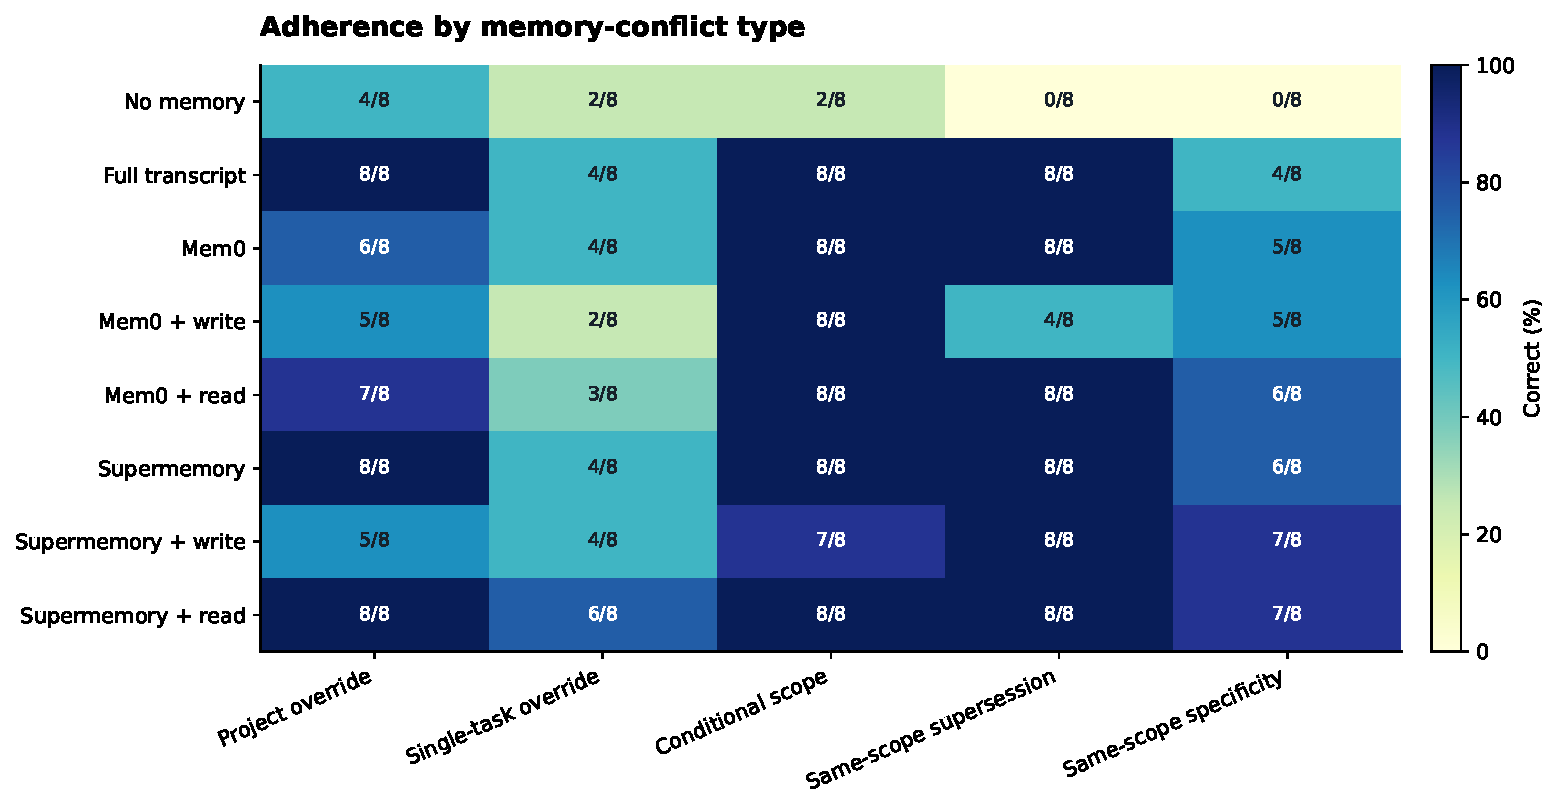
\includegraphics[width=\linewidth]{04_conflict_heatmap.pdf}
\caption{Adherence across five conflict categories;
eight episodes per category.}
\label{fig:conflict-types}
\end{minipage}
\end{figure}

Across conflict types (Figure~\ref{fig:conflict-types}),
conditional scope and same-scope supersession are
handled reliably by most memory-system conditions.
Single-task overrides are hardest: Mem0 and
Supermemory each achieve 4/8, while read-time
Supermemory reaches 6/8. Same-scope specificity
also remains challenging, with 4--7/8 correct
among the full-transcript and memory conditions.


\subsection{Failure Diagnosis, Tagging, and Retention}

The diagnostic breakdown in
Figure~\ref{fig:failure-stages} (Appendix~\ref{app:metrics}) attributes most
Supermemory baseline errors to reasoning despite
available information. Mem0 exhibits five baseline
scope-loss errors; write-time Mem0 has seven
extraction and four tagging failures among its
16 incorrect responses. Supermemory + write-time
has eight reasoning-classified failures among nine.

Write-time tagging achieves 100\% scope accuracy
on evaluated tags for both systems, versus 87\%
for read-time Mem0 and 77\% for read-time
Supermemory. Nevertheless, the highest downstream
adherence occurs with read-time Supermemory,
illustrating that tag accuracy alone is insufficient.
These figures use different eligible-note sets
and are not directly controlled comparisons.

Unrelated-memory retention is 95\% with the full
transcript, 67.5\% with Mem0 (significantly lower,
$p=0.003$), and 97.5\% with Supermemory. Scope-aware
Mem0 variants retain 62--72\%, compared with 87--98\%
for Supermemory variants; tagging does not change
retention significantly for either system.


% ====================
% 6. Analysis of results, failures, limitations, costs, and risks
% ====================
\section{Analysis of Results, Failures, Limitations, Costs, and Risks}
\label{sec:discussion}

\subsection{Write-Time versus Read-Time Tagging}

Read-time tagging matches or improves adherence
relative to both memory-system baselines, whereas
write-time tagging reduces it. One possible
explanation is that write-time extraction isolates
instructions from conversational context, making
task continuity difficult to infer. Conversely,
read-time tagging retains the underlying memory
system's representation, although its tags may
be less accurate. Write-time Supermemory illustrates the
trade-off: it never over-applies a scoped memory (20/20
out-of-scope probes) but often fails to apply one when it
should.


\subsection{Why Retrieval and Tagging Are Insufficient}

The retrieval--application gap shows that access
to a relevant instruction does not ensure correct
conflict resolution. In pair \texttt{po-01}, for
example, an agent may select the standing Polars
preference despite the applicable project-specific
pandas instruction. Other failures involve
carrying a single-task exception into a new task
or combining conflicting instructions.

Effective memory thus requires both relevant information and
reliable contextual decision-making; representative examples
are in Appendix~\ref{app:failure-cases}.

\subsection{Threats to Validity}

The benchmark contains only 20 synthetic pairs with short
histories and explicit scope cues; 19 were initially
AI-assisted, and numeric conditions avoid threshold
boundaries. Findings may not generalize to longer, ambiguous,
or naturally occurring interactions. The study uses one agent
model and one run per condition; fixed sampling settings do
not guarantee reproducibility, and Supermemory's hosted
processing is not fully observable.

The scope treatments change three components at once: scope
tags, conflict-resolution rules, and memory ordering (oldest
first, versus relevance order without timestamps for the
baselines). Differences therefore cannot be attributed to
tags alone; the non-significant gain for read-time Supermemory
(37/40 versus 34/40; McNemar $p=0.25$) may arise from the
rules or ordering. Rules-only, tags-only, and ordering-only
ablations would isolate these contributions.

Retrieval matching and failure-stage diagnoses were not
independently validated in full, and the two probes within
each pair are dependent, limiting episode-level significance
tests.

\textbf{Cost.} OpenRouter spending for the full experiment was
about \$0.15 (about \$0.06 for judging); Supermemory's separately
billed processing is excluded.

% ====================
% 7. Reproducibility and responsible practice
% ====================
\section{Reproducibility and Responsible Practice}
\label{sec:reproducibility}

Code, the 320 run logs, and cached judge verdicts are in the public
repository, so results can be rescored without new agent calls
(Appendix~\ref{app:reproducibility}).

\subsection{Ethical Considerations and Risks}

This study poses limited direct risk: all sessions and probes
are synthetic (mainly coding, data, and email tasks), and no
real user data were collected or sent to OpenRouter or
Supermemory. Two risks would matter in deployment.

\textbf{Misapplied memory.} An agent that carries an
instruction beyond its intended scope, or fails to apply
it within scope, may act against the user's wishes, which
matters most for privacy, safety, or permissions (``do not
email this person''). Deployments should require human
confirmation before consequential memory-driven actions.

\textbf{Memory poisoning.} Session text and retrieved
memories are passed to the tagger and agent without
filtering. Malicious notes, such as ``ignore previous
rules,'' could steer either component. Our benchmark contains no adversarial memories, so we cannot
assess robustness to poisoning; deployed systems should treat
stored memories as untrusted content that cannot override
higher-priority rules.


% ====================
% 8. Conclusion
% ====================
\section{Conclusion}
\label{sec:conclusion}

Across 320 runs, agents frequently misapplied
memories even when the expected memory was retrieved.
Read-time tagging with Supermemory achieved the
highest observed adherence, while write-time
tagging reduced performance for both memory
systems. The results suggest that scope-aware
interventions can be useful, but explicit
metadata alone does not resolve contextual
memory conflicts. Larger benchmarks and
controlled ablations are needed to isolate
the effects of tagging, conflict-resolution
instructions, and memory ordering.



% ====================
% End of main text (8-page limit)
% ====================
\clearpage

% ====================
% Contribution statement (not counted toward the page limit)
% ====================
\section*{Contribution Statement}

\begin{center}
\begin{tabular}{@{}>{\raggedright\arraybackslash}p{0.28\linewidth}
                >{\raggedright\arraybackslash}p{0.52\linewidth}
                >{\centering\arraybackslash}p{0.12\linewidth}@{}}
\toprule
\textbf{Member (Student ID)} & \textbf{Main contributions} & \textbf{Share (\%)} \\
\midrule
Isaac Chin Wei En (A0248885H) &
Environment and baseline integration; episode schema, scope-labelling
guide and 20-pair benchmark; automated validation and leakage checks;
agent-model selection pilot & 25 \\
Edward Chew Kian Boon (A0271710N) &
Implemented write-time and read-time scope-tagging integration, memory
retrieval, and episode-level storage and retrieval logging & 25 \\
Ng Cheng Kiat Nicholas (A0271938R) &
Built evaluation infrastructure, configured experimental conditions,
implemented scoring and LLM-as-a-judge evaluation, and generated
experimental run results & 25 \\
Jagan Mohan Shailesh (A0272542H) &
Gold-label annotation and adjudication; experimental result validation
and rescoring; statistical analysis and visualization; qualitative
failure analysis; \LaTeX{} preparation & 25 \\
\midrule
\textbf{Total} & & \textbf{100} \\
\bottomrule
\end{tabular}
\end{center}


% References (not counted toward the page limit)
\bibliographystyle{plainnat}
\bibliography{refs}

% Appendix (not counted toward the page limit)
\appendix
% ====================
% Appendix (not counted toward the page limit)
% ====================

\section{Episode Examples and Qualitative Failure Analysis}
\label{app:failure-cases}

\subsection{Episode JSON Structure}
\label{app:episode-schema}

Each benchmark pair is stored as a JSON file under
\path{episodes/pairs/}. The file contains the shared
conversation history, reference memories, two evaluation
probes, and an unrelated-memory retention check.
Table~\ref{tab:episode-schema} summarises the top-level
fields.

\begin{table}[htbp]
\centering
\small
\caption{Top-level fields of an episode-pair JSON file.}
\label{tab:episode-schema}
\begin{tabularx}{\linewidth}{lX}
\toprule
Field & Description \\
\midrule
\texttt{pair\_id} &
Unique identifier of the paired scenario. \\

\texttt{conflict\_type} &
Type of memory conflict being evaluated. \\

\texttt{domain} &
Specific decision domain, such as dataframe library. \\

\texttt{domain\_kind} &
Broader category of the task domain. \\

\texttt{sessions} &
Ordered earlier conversations containing user
instructions and contextual information. \\

\texttt{memories} &
Reference instructions extracted from the sessions,
including their source, role, intended action,
and gold scope annotations. \\

\texttt{probes} &
Two evaluation tasks (A and B) sharing the same
history but differing in contextual applicability.
Each specifies its expected action and winning memory. \\

\texttt{retention\_checks} &
Requirements testing whether unrelated standing
preferences are preserved. \\
\bottomrule
\end{tabularx}
\end{table}

Each session contains a \texttt{session\_id},
chronological \texttt{order}, \texttt{task\_id},
\texttt{active\_project}, and conversation
\texttt{text}.

Each reference memory contains a \texttt{memory\_id},
source \texttt{session\_id}, instruction \texttt{text},
\texttt{role}, \texttt{decision}, \texttt{action},
and a \texttt{gold} object. The latter specifies
\texttt{scope}, \texttt{key}, and \texttt{condition}.

Each probe contains a task identifier, project context,
natural-language request, structured \texttt{facts},
an \texttt{in\_scope} indicator, the decision being
tested, \texttt{expected\_action},
\texttt{expected\_memory}, and \texttt{deciding\_rule}.

The \texttt{retention\_checks} array identifies
an unrelated memory and the requirement used
to evaluate whether it is followed.

Only the conversation sessions and the selected
probe text are supplied as episode inputs to
the experimental systems. Reference memories,
structured context, gold labels, and expected
outcomes are reserved for validation and scoring.

\subsection{Complete Example: Project Override
(\texttt{po-01})}
\label{app:po01-example}

Pair \texttt{po-01} illustrates the mirrored-pair
design. Two earlier sessions establish three
reference memories: a standing preference for
Polars on datasets exceeding one million rows,
a project-specific instruction to use pandas
for Project Marlin, and an unrelated requirement
for Python type hints.

Probe A concerns Project Marlin, where the
project-specific instruction takes precedence.
Probe B changes only the project to Project Tern,
where the standing Polars preference applies.
Both probes independently test retention of
the type-hint instruction.

Figure~\ref{fig:mirrored-pair} summarises this structure,
and Listing~\ref{lst:po01} reproduces the complete
JSON specification used by the benchmark.

\begin{figure}[H]
\centering
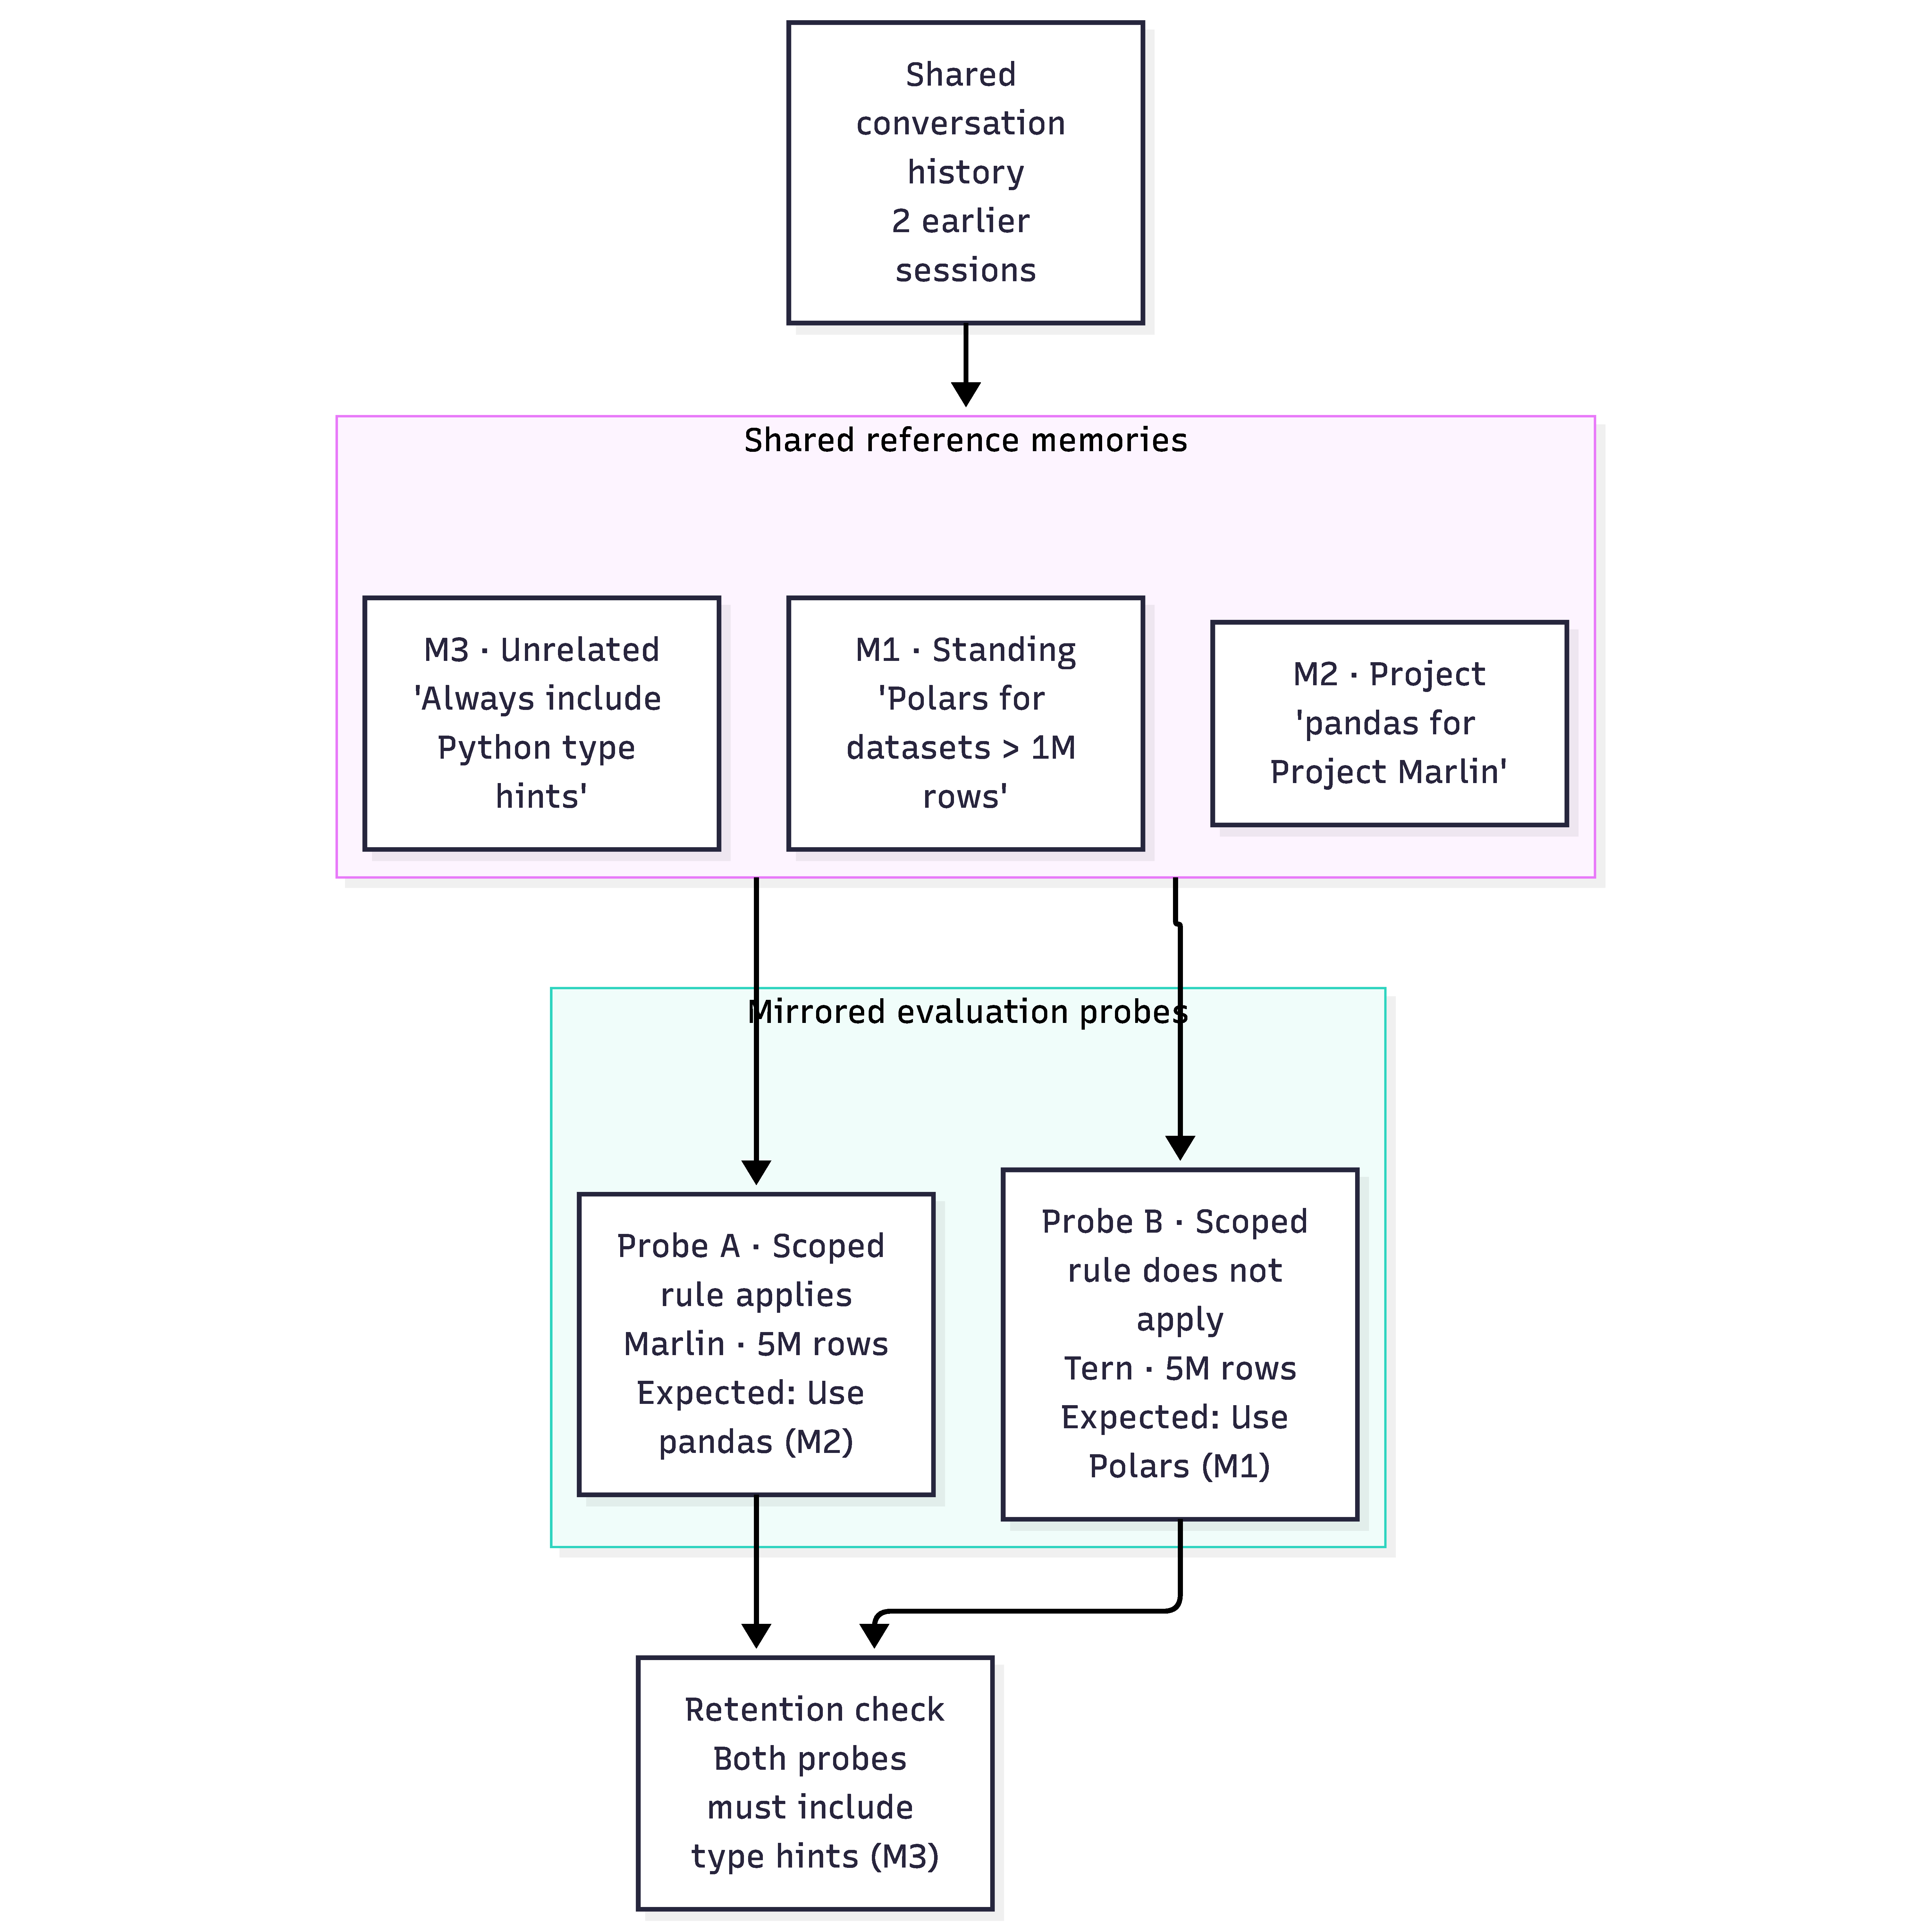
\includegraphics[width=0.4\linewidth]{mirrored_pair_design.pdf}
\caption{Mirrored-pair benchmark design illustrated
    using pair \texttt{po-01}. Both probes share the
    same conversation history and reference memories
    but differ in whether the project-specific instruction
    applies. An unrelated standing preference is
    evaluated independently in both probes.}
\label{fig:mirrored-pair}
\end{figure}

\begin{lstlisting}[style=jsonstyle,
    caption={Complete JSON specification of
    project-override pair \texttt{po-01}.},
    label={lst:po01}]
{
  "pair_id": "po-01",
  "conflict_type": "project_override",
  "domain": "dataframe library",
  "domain_kind": "developer",
  "sessions": [
    {
      "session_id": "s1",
      "order": 1,
      "task_id": "t-po01-1",
      "active_project": "Project Marlin",
      "text": "User: I'm kicking off Project Marlin, a nightly sales rollup for the finance team. For Project Marlin, use pandas. My teammate only knows pandas.\nAssistant: Understood, pandas for Marlin. What does the first job look like?\nUser: It reads a CSV with an order_date column written day/month/year. How should I parse those dates?\nAssistant: Tell the parser the day comes first, for example with dayfirst=True, and then check a few rows around the 12th of each month.\nUser: That works. I'll come back with the next job."
    },
    {
      "session_id": "s2",
      "order": 2,
      "task_id": "t-po01-2",
      "active_project": null,
      "text": "User: Our load script reads a big CSV and takes ages. Any quick wins?\nAssistant: Read only the columns you need and give the parser explicit column types. Here is a sketch: def load(path): return read_csv(path, usecols=['id', 'total'])\nUser: That snippet had no type hints. Whenever you write a function for me, give every parameter and the return value a type hint.\nAssistant: Sorry about that. From here on every function I write will have type hints on its parameters and its return value.\nUser: On the library question, I usually go with Polars when a dataset is over 1M rows.\nAssistant: Got it. I'll keep that in mind for large datasets.\nUser: Thanks, that's all for now."
    }
  ],
  "memories": [
    {
      "memory_id": "m1",
      "session_id": "s2",
      "text": "I usually go with Polars when a dataset is over 1M rows.",
      "role": "standing",
      "decision": "dataframe_library",
      "action": "polars",
      "gold": {
        "scope": "standing",
        "key": null,
        "condition": "rows > 1000000"
      }
    },
    {
      "memory_id": "m2",
      "session_id": "s1",
      "text": "For Project Marlin, use pandas.",
      "role": "scoped",
      "decision": "dataframe_library",
      "action": "pandas",
      "gold": {
        "scope": "project",
        "key": "Project Marlin",
        "condition": null
      }
    },
    {
      "memory_id": "m3",
      "session_id": "s2",
      "text": "Whenever you write a function for me, give every parameter and the return value a type hint.",
      "role": "unrelated",
      "decision": null,
      "action": null,
      "gold": {
        "scope": "standing",
        "key": null,
        "condition": null
      }
    }
  ],
  "probes": {
    "A": {
      "task_id": "t-po01-3",
      "active_project": "Project Marlin",
      "text": "Write a Python function that deduplicates the 5M-row orders table for Project Marlin by order_id, keeping the row with the latest updated_at, and returns the cleaned dataframe.",
      "facts": {
        "rows": {
          "value": 5000000,
          "text": "5M-row"
        }
      },
      "in_scope": true,
      "decision": "dataframe_library",
      "expected_action": "pandas",
      "expected_memory": "m2",
      "deciding_rule": 2
    },
    "B": {
      "task_id": "t-po01-4",
      "active_project": "Project Tern",
      "text": "Write a Python function that deduplicates the 5M-row orders table for Project Tern by order_id, keeping the row with the latest updated_at, and returns the cleaned dataframe.",
      "facts": {
        "rows": {
          "value": 5000000,
          "text": "5M-row"
        }
      },
      "in_scope": false,
      "decision": "dataframe_library",
      "expected_action": "polars",
      "expected_memory": "m1",
      "deciding_rule": 1
    }
  },
  "retention_checks": [
    {
      "memory_id": "m3",
      "check": "The function in the agent's code has a type hint on every parameter and on the return value"
    }
  ]
}
\end{lstlisting}

\subsection{Qualitative Failure Cases}
\label{app:qualitative-failures}

The following cases illustrate distinct
memory-application failures observed in the
experimental evaluation.

\subsubsection{Project Override:
\texttt{po-01}}

The user generally prefers Polars for datasets
exceeding one million rows but requires pandas
for Project Marlin.

Probe A concerns Marlin and expects pandas,
whereas Probe B concerns Project Tern and
expects Polars. The unrelated type-hint
preference applies to both.

On Probe A, four conditions chose Polars where
pandas was expected: Mem0, both scope-tagged Mem0
variants, and write-time scope-tagged Supermemory.
In all four, the Marlin pandas instruction was among
the retrieved memories, and the failure was in the
agent's reasoning. Plain Mem0 opened its answer with
``Use Polars for this 5M-row dataset to ensure high
performance and memory efficiency.'' In both tagged
Mem0 variants, the tagger had labelled the Marlin
memory as project scope with key Project Marlin and
the Polars memory as standing scope, yet the agent
still applied the standing rule.

The full-transcript, Supermemory and read-time
scope-tagged Supermemory conditions chose pandas on
Probe A. All seven conditions with memory chose Polars
on Probe B, as expected. Retrieving the applicable
instruction therefore did not ensure that the agent
applied it over a conflicting standing preference.

\subsubsection{Single-Task Override:
\texttt{st-04}}

The user generally prefers inline SQL subqueries,
requires common table expressions (CTEs) for
Project Marlin, and requests views for one
particular task.

Probe A concerns the task for which views were
requested and therefore expects views. Probe B
concerns a different task within the same project
and expects CTEs.

Some conditions incorrectly carry the single-task
exception into Probe B, while others fail to
apply it in Probe A. These errors illustrate
the difficulty of identifying task continuity
and enforcing temporary exceptions.

\subsubsection{Same-Scope Specificity:
\texttt{sp-02}}

The user normally begins emails with
``To whom it may concern,'' but prefers
``Hey there,'' when writing to a neighbour.

Probe A concerns a neighbour and expects
the conditional greeting. Probe B concerns
a landlord and expects the default greeting.

Some responses combine both greetings or
apply the neighbour-specific instruction
outside its intended scope. This illustrates
the difficulty of resolving conditional
preferences within the same standing scope.

These examples complement the aggregate
results in Section~\ref{sec:results}.
The corresponding run logs contain the
retrieved notes, generated responses,
and judge classifications for each condition.


\section{Supplementary Experimental Results}
\label{app:supplementary-results}

Figure~\ref{fig:conflict-types} breaks adherence down by
conflict category.

\begin{figure}[H]
\centering
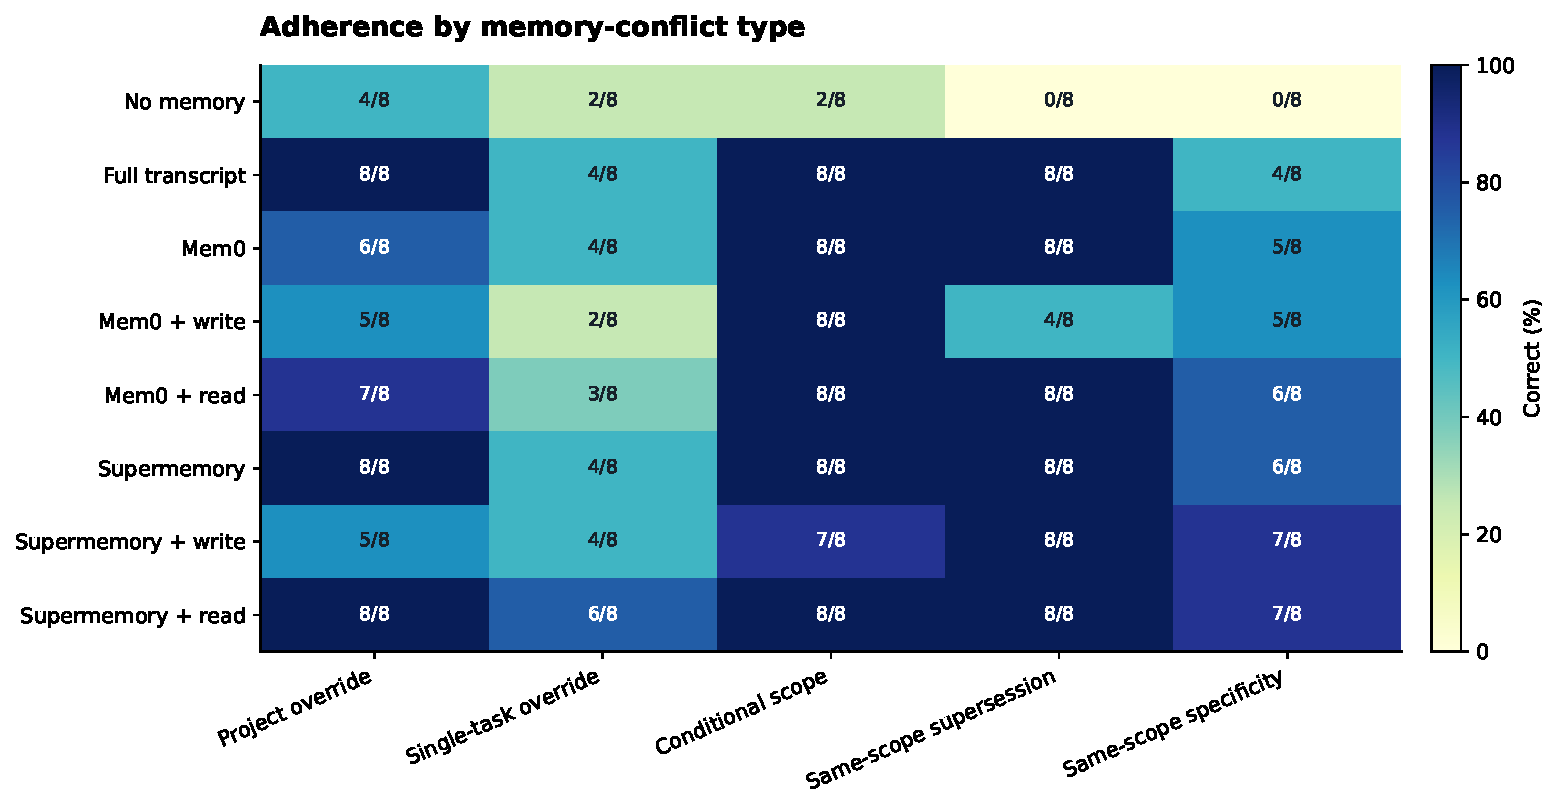
\includegraphics[width=0.6\linewidth]{04_conflict_heatmap.pdf}
\caption{Adherence across five conflict categories;
eight episodes per category.}
\label{fig:conflict-types}
\end{figure}

The full pair-by-pair adherence matrix,
tagging-accuracy breakdown, failure-stage
counts, and per-condition cost accounting
are available in \texttt{reports/summary.md}
and \texttt{reports/episode\_scores.csv}.

OpenRouter spending for the full experiment
was approximately \$0.15, with approximately
\$0.06 for judging. Supermemory's separately
billed processing is excluded.

\paragraph{Metric details.} Incorrect decisions are
classified as over-application, under-application,
supersession, or other actions.
Retrieval is checked by verbatim matching or
judge-assisted matching of rewritten notes. The
full-transcript control counts as successful retrieval
by construction; no memory counts as unsuccessful.
Retention excludes unassessable answers.

Tagging accuracy is measured on notes associated with
one reference memory. Scope is matched exactly;
project keys must contain the reference project name,
while single-task keys are excluded from scoring.
Conditions use strict (variable, operator, value)
and lenient (operator, value) matching.

Failure-stage categories are extraction, retrieval,
scope loss, tagging, and reasoning. Each incorrect
answer is assigned to the earliest detected failure.
These are diagnostic classifications, not established
causal mechanisms. Supermemory's internal extraction
cannot be inspected separately from retrieval.

\section{Reproducibility and Implementation Details}
\label{app:reproducibility}

The implementation is available in the project
repository. Experimental conditions are defined
in \texttt{agent/conditions.py}; runs are executed
through \texttt{agent/runner.py}; and scoring is
implemented in \texttt{scoring/}.

All 320 runs completed without execution errors.
The 320 existing run logs, cached judge verdicts,
and cost ledger allow rescoring without repeating
agent calls. Figures are generated from the
scoring outputs in \texttt{reports/}.

\paragraph{Model selection.} Qwen was selected after an
operational pilot: it reported zero reasoning usage on
40 pilot calls, whereas DeepSeek returned empty text on
three of eight calls when reasoning was disabled.

\paragraph{Memory-system configuration.} Mem0 uses its
default extraction and search, an
\texttt{all-MiniLM-L6-v2} embedder (384 dimensions),
Qdrant storage, and internal LLM calls through
OpenRouter. The base \texttt{mem0ai} installation
excludes optional spaCy and fastembed dependencies;
the initial smoke test used vector retrieval without
BM25. Supermemory uses its hosted API and waits for
ingestion to complete before retrieval.

\paragraph{Cost logging.} OpenRouter token usage and
costs are recorded in an append-only ledger.
Supermemory's separately billed processing is excluded
from those costs.


\end{document}
